\chapter{Detector and Focal Plane Design}\label{c:det-design}

This chapter describes the design of the \Imager's detectors and focal plane.
It begins with a discussion of the choice of parameters $G$, $C$, $T_c$ and $T_b$ for the detectors, followed by details of the detector design used to achieve these parameters.
I then briefly describe the design of the focal plane, and end with the predicted detector noise and \NETD\ for the system.

\section{Parameter Choice For Our Bolometers} \label{sec:det-parm-choice}

The primary parameters to be chosen when designing a \TES\ bolometer are the superconducting critical temperature $T_c$, the thermal conductance $G$, and the \TES\ island heat capacity $C$.
These parameters are interrelated, and so cannot be chosen entirely independently of each other.
Some of the factors to consider are:
\begin{itemize}
  \item Detector noise scales with $\sqrt{T_c^2 G}$, so that lower values of $G$ and $T_c$ improve noise
  \item The saturation power of the \TES\ detector scales roughly like $G T_c$, so that if $G$ and $T_c$ are too small, the optical power falling on the detector will raise the temperature of the membrane above $T_c$, causing the device to not work.
    % do i talk about saturation power in ch 3? if not, I should!
  \item $T_c$ must be chosen to be higher than the achievable bath temperature, and the bath temperature also affects the saturation power through \eqnref{eqn:ch3-p-bath}.
  \item The detector time constant $\tau_{eff}$ is proportional to the detector natural time constant $\tau = C / G$.
\end{itemize}

% xxx say something about no attempt to shape transition - we get whatever alpha we get. no need to slow down trans, which is what normal metal bars do.

The following subsections outline the choice of $T_b$, $T_c$, $G$ and $C$ for the detectors in the first 251-detector sub-array.

\subsection{Choice of $T_b$ and $T_c$}

The relationship between detector noise and saturation power can be examined in more detail.
From \eqnref{eqn:ch3-g-fit} we have
\begin{equation} \label{eqn:ch5-psat}
P_{sat} = \frac{G T_c}{n}\left(1 - \left(\frac{T_b}{T_c}\right)^n\right).
\end{equation}
This can be solved for $G$ and substituted into the expression for \TES\ thermal fluctuation noise in \tableref{tab:tes-noise}, leading to
\begin{equation} \label{eqn:ch5-tes-noise}
S^2_{TFN} = \frac{n F(T_0, T_b) T_0 / T_b}{1-(T_b/T_c)^n} 4 \, k_B T_b P_{sat}.
\end{equation}
The \TES\ temperature $T_0$ appears only in the pre-factor, which depends only on the power-flow index $n$, the ratio $T_b/T_0$, and the form of $F$.
This means that for fixed $P_{sat}$ and $T_b$, the ratio $T_c/T_b$ that gives the lowest detector noise depends only on $n$ and the form of $F$.
For values of $n$ in the range 3--4, this optimal ratio is $T_c \approx 1.8 T_b$, while the pre-factor itself is \abt{3.7}.

As discussed in \sectionref{sec:ch4-opt-eff}, the predicted loading on the \Imager's detectors is \SI{180}{\pW} and the photon noise from this load is \Pnoisef{0.85}.
Choosing a safety factor of 3 so that $P_{sat} = 3 \times \SI{180}{\pW}$, and targeting detector noise equal to \SI{50}{\percent} of the photon noise (so that total noise is a factor of $\sqrt{1.5} = 1.22$ higher than photon noise), we find that in order for the detector noise to be below the predicted photon noise we require
\begin{equation}
  T_b < \frac{1}{3.7} \frac{\NEPph^2}{4 k_B P_{sat}} =
        \frac{1}{3.7} \frac{0.5 \times (\num{0.85e-15})^2}{4 \times \SI{1.38e-23}{\J\per\K} \times 3 \times \SI{180}{\pW}} = 
        \SI{3.6}{\K}
\end{equation}
It would seem that we should be able to run the system off of a Pulse Tube Cooler.

However, this leaves little margin for error in the design and implementation of the system, so for the \Imager\ we chose to use a \He4-sorption fridge to set the bath temperature.

The initial hopes for performance of the \He4-sorption fridge were that it's base temperature would be ~\SI{650}{\mK}, implying an ideal $T_c$ of \abt{\SI{1.2}{\K}}.
This is a convenient $T_c$ because it is the critical temperature of elemental Al \cite{matthias_superconductivity_1963}, so Al was chosen as the \TES\ material.

In practice, it was discovered during testing of Al prototype detectors that the base temperature of the system was \SI{950}{\mK} under optical load, so that a higher $T_c$ could lead to better noise performance.
However, in order to change as little as possible between the prototype detectors and the first sub-array, I decided to continue using Al.

\subsection{Choice of $G$}

\tableref{tab:ch5-proto-parms} lists the measured properties and parameters of the prototype detectors.
These detectors had $P_{sat}$ at $T_b = \SI{970}{\mK}$, 5.1 times higher than the predicted optical load and 6.1 times the measured optical load.
A safety factor of 5--6 is overly conservative, so for the sub-array I decided to target a $G$ value of \SI{3.8}{\nW\per\K}, for a safety factor of 3.9 -- 4.7.

\begin{table*}
\centering
\caption[Measured properties of prototype detectors]{
  Measured Properties of Prototype Detectors.
  The methods and procedures used to measure these properties were the same as described for the sub-array in \chapterref{c:det-array}.
} 
\label{tab:ch5-proto-parms}
\begin{tabular}{l c}
\toprule
  Detector Property &  {Value} \\
\midrule
  $T_c$                 & \SI{1.2}{\K} \\
  $R_n$                 & \SI{3.4}{\mOhm} \\
  $n$                   & 3.9 \\
  $G$                   & \SI{5}{\nW\per\K} \\
  $\tau$                & \SI{12}{\ms} \\
  $\tau_{eff}$ (typical) & \SI{4}{\ms} \\
  $C = G \tau $         & \SI{60}{\pJ\per\K} \\
  $P_{opt}$              & \SI{150}{\pW\per\K} \\
  $\eta_{tot}$           & 0.25 \\
  $P_{sat}|_{\SI{970}{\mK}}$          & \SI{920}{\pW} \\
\bottomrule
\end{tabular}
\end{table*}

\subsection{Choice of $C$}

The detector's heat capacity $C$ is chosen to target a specific natural time constant $\tau$ once $G$ is chosen.
$\tau_{eff}$ in the prototype detectors was higher than the desired value of \SI{1}{\ms} (see \sectionref{sec:ch2-specifications}).
To reduce the risk of problems such as instability with the sub-array detectors, I decided to reduce $C$ to \SI{30}{\pJ\per\K}, which would give $\tau = \SI{8}{\ms}$.
As long as \Loop and $\beta_I$ at the operating bias point did not change, this would lead to $\tau_{eff} = \SI{2.6}{\ms}$, not as fast as would be ideal, but fast enough for video imaging

\section{Detailed Detector Design} \label{sec:ch5-det-design}

The \Imager's detectors are fabricated using standard lithographic clean-room techniques on Si wafers.
In order to achieve the targeted $G$ and $C$ values the detectors are located on a suspended SiN membrane which is connected to the rest of the Si wafer by a set of thin ``legs''.
\figref{fig:ch5-det-layout} shows a cross-sectional schematic of the detectors, showing that they are suspended with no Si beneath them, as well as a labeled photograph of a prototype detector.
The sub-array detectors are identical except for the length of the legs and the thickness of some of the layers; see \tableref{tab:ch5-det-dims}.

\begin{figure*}
\centering
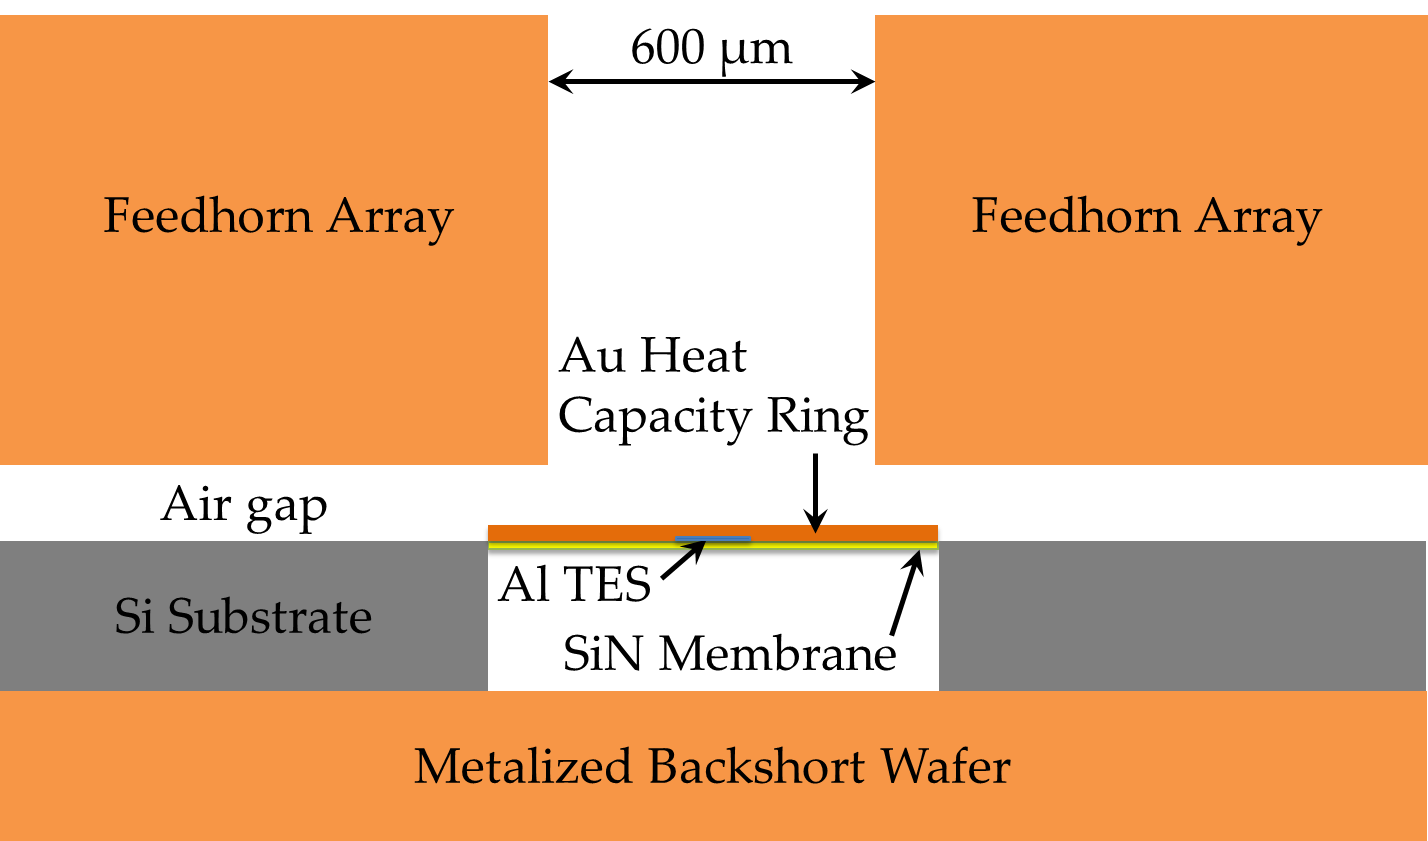
\includegraphics[width=3.9in]{images/ch5-det-schematic.png}
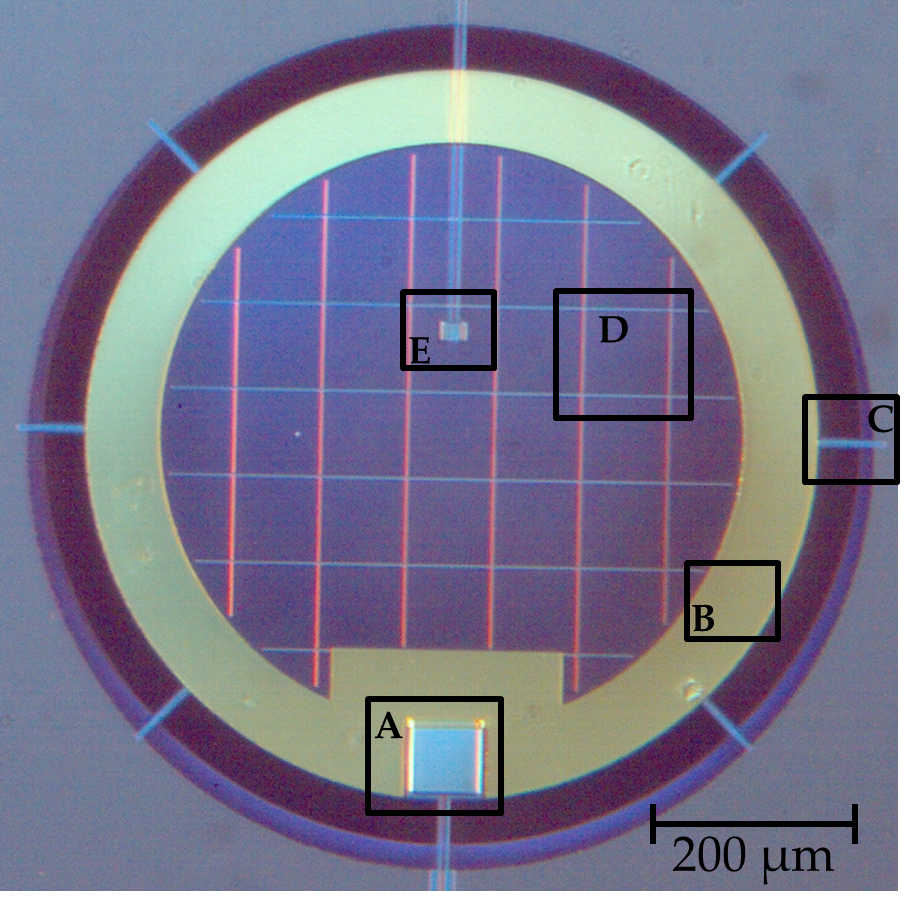
\includegraphics[width=2.3in]{images/ch5-proto-pixel-labeled.png}
\caption[Detector cross-section and photograph]{
  \textbf{Left} Cross-sectional schematic of a \Imager\ detector.
  The schematic is not to scale.
  \textbf{Right} Photograph of a prototype detector.
  The detectors fabricated for the sub-array are identical except for the length of the legs and the thickness of some of the layers; see \tableref{tab:ch5-det-dims}.
  The labeled parts of the detector are \textbf{A} Al \TES\ \textbf{B} Au heat capactiy ring \textbf{C} SiN leg connecting detector to substrate \textbf{D} PdAu absorbing mesh \textbf{E} PdAu heater resistor.
}
\label{fig:ch5-det-layout}
\end{figure*}

The detectors are fabricated on \SI{275}{\um} thick double-side-polished degenerate (Boron P-type) Si wafers.
A layer of SiO2 is grown on top of the silion, followed by a layer of SiN, prior to the main fabrication steps.
During fabrication the Nb wiring leads, PdAu absorber, and Au heat-capacity ring are laid down, as well as an additional layer of insulator to allow wiring layers to cross over each other.
The SiN and SiO2 is removed from the areas between the legs, and then a Deep Reactive Ion Etch process is used to remove all silicon from behind the detector membrane.
This etch process does not remove SiN or SiO2, so that the legs, which still have SiN, are left in place.
The result is a suspended membrane connected to the rest of the wafer by a set of ``legs'' which provide the thermal conductance $G$.

\tableref{tab:ch5-det-dims} lists dimensions for both the prototype and sub-array detectors.

The leg geometry of the prototype detectors was based on a set of measurements taken at \NIST\ on SiN membranes at temperature around \SI{1}{\K}.
the leg geometry for the sub-array detectors was based on simple scaling of the prototype detectors to the target $G$ of \SI{3.8}{\nW\per\K}.
This scaling was slightly complicated by the change in thickness of the SiO2 layers, which was made in order to add additional protection to the wiring laayers and better balance stress on the relieved membranes.
Assuming that $G$ scales linearly with the $A/L$ of the legs, the sub-array $G$ should be
\begin{align}
  G_{sub} & = G_{proto} \frac{A_{sub}}{A_{proto}} \frac{l_{proto}}{l_{sub}} \\
         & = G_{proto} \frac{(500 + 250 + 200)(11)}{(500 + 120 + 120)(11)} \frac{40}{67} \\
         & = \SI{5.0}{\nW\per\K} \times 1.28 \times 0.597 \\
         & = \SI{3.8}{\nW\per\K} 
\end{align}

\begin{table*}
\centering
\caption[Detector dimensions]{
  Dimensions of prototype and sub-array detectors.
  For the sub-array, only values differing from the protottypes are shown.
} 
\label{tab:ch5-det-dims}
\begin{tabular}{l c c}
\toprule
  Detector Dimension &  {Prototype} & Sub-Array \\
\midrule
  \TES\ Size           & $\SI{64}{\um} \times \SI{70}{\um}$ & \\
  \TES\ Thickness      & \SI{250}{\nm}       & \SI{180}{\nm} \\
  SiN Thickness        & \SI{500}{\nm}       & \\
  SiO2 Base Thickness  & \SI{120}{\nm}       & \SI{250}{\nm} \\
  SiO2 Cover Thickness & \SI{120}{\nm}       & \SI{200}{\nm} \\
  Number of Legs       & 8                   & \\
  Leg Length           & \SI{40}{\um}        & \SI{67}{\um} \\
  Leg Width            & \SI{11}{\um}        & \\
  Gold Ring Area       & $(\SI{393}{\um})^2$ & \\
  Gold Ring Thickness  & \SI{2000}{\nm}      & \SI{1000}{\nm} \\
  Nb Lead Width        & \SI{6}{\um}         & \\
  Nb Lead Thickness    & \SI{200}{\nm}       & \\
  PdAu Thickness       & \SI{20}{\nm}        & \\
\bottomrule
\end{tabular}
\end{table*}

\tableref{tab:ch5-det-heat-capacity} shows contributions to the heat capactiy from all components of the bolometer.
The membrane and Al \TES\ alone have insufficient heat capacity, so an Au ring was added to provide the targetted heat capacity.
The total heat capacity is dominated by the Au ring.

\begin{table*}
\centering
\caption[Detector heat capacity contributions]{
  Contributions to total heat capacity of sub-array detectors.
  Note that the Debye $T^3$ contribution for Au is still significant at \SI{1.2}{\K}, so must not be ignored.
  All values listed are at \SI{1.2}{\K}.
} 
\label{tab:ch5-det-heat-capacity}
\begin{tabular}{l S S S l}
\toprule
  Component & {Volume ($10^{-9}$\,\si{\cm^3})} & {$C_V$ (\si{\uJ\per\K\per\cm^3})} & {$C_{tot}$ (\si{\uJ\per\K})} & Source \\
\midrule 
    SiN & 203.6 &   1.0 &   0.2 & \cite{holmes_measurements_1998} \\ 
   SiO2 & 183.2 &   3.1 &   0.6 & \cite{zeller_thermal_1971,zink_specific_2004} \\ 
     Al &   0.8 & 196.8 &   0.2 & \cite{irwin_transition-edge_2005} \\ 
     Au & 154.4 & 161.3 &  24.9 & \cite{corak_atomic_1955} \\ 
\midrule 
  Total &       &       &  25.8 \\ 
\bottomrule
\end{tabular}
\end{table*}

\section{Detector Wafer Layout} \label{sec:ch5-layout}

\figref{fig:ch5-full-wafer} shows a photograph of the entire sub-array; the figure caption contains a detailed description of the features present on the sub-array.
In addition to the detectors, the wafer includes Au pads for attaching Au heat-sinking wire bonds and holes used for glueing the detector wafer to a Au-covered backshort wafer (see \sectionref{sec:ch5-focal-plane}).
Note that all detectors have heater resistors on their membranes, but only a subset have the resistors connected to wires that lead to bondpads.

The detectors are laid out on a square grid, chosen over a hexagonal close-packed layout because of the simpler wiring layout.
This choice does worsen \NETD.
A hexagonal close-packed array would allow the same number of detetors to be placed on the array, but with feedhorns \SI{7.5}{\percent} larger.
The larger feedhorn size could have improved the spill over effieciency from \num{0.52} to \num{0.544}, a \SI{4.6}{\percent} increase, leading to a \SI{4.6}{\percent} improvement in \NETD.

\begin{figure*}
\centering
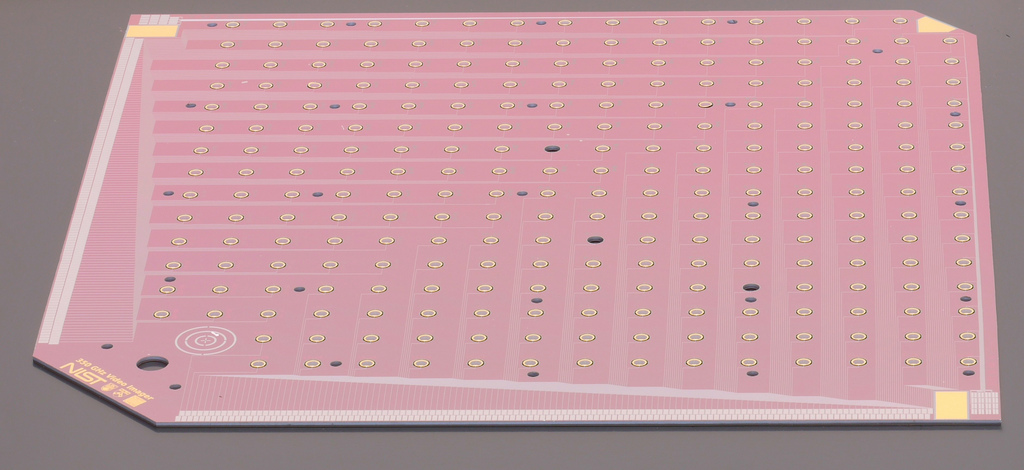
\includegraphics{drawings/ch5-full-wafer.pdf}
\caption[Photograph of 251-detector sub-array]{
  Photograph of the 251-detector sub-array.
  Bondpads for connecting to the detectors run along the left and bottom sides.
  In the upper left, lower right, and upper right corners are Au pads for connecting Au wirebonds to allow the wafer to be heat-sunk to the rest of the \SI{1}{\K} stage.
  The upper left and lower right corners also contain small bondpads for connecting to detector heaters.
  While all detectors have heater resistors on their membrane, only the detectors along the upper and right edges have these resistors wired to bondpads.
  The 26 small holes spaced throughout the wafer are used to glue the detector wafer to a backshort wafer (see text).
  The three larger holes in the middle of the wafer are detector sites where the membrane was broken during fabrication.
  The large hole in the lower left, as well as the ``bulls-eye'' feature to its immediate upper right, were intended to be used as alignment features, although the alignment procedure actually used did not use these features.
  Photograph credit Dan Schmidt; full-resolution version available at \protect\url{http://www.flickr.com/photos/quantumsensors/8592792487}.
}
\label{fig:ch5-full-wafer}
\end{figure*}

\section{Focal Plane Design} \label{sec:ch5-focal-plane}

The \Imager's detector arrays are mounted on an Al platter that is thermally sunk to the cold head of the \He4-sorption fridge via a set of Cu ropes.
Mechanically the focal plane is attached to an Al frame via four Ti-6Al-4V ``spiders''.
The frame itself is bolted to the \SI{6}{\K} cold plate.
See \figref{fig:ch5-focal-plane-back}.

\begin{figure*}
\centering
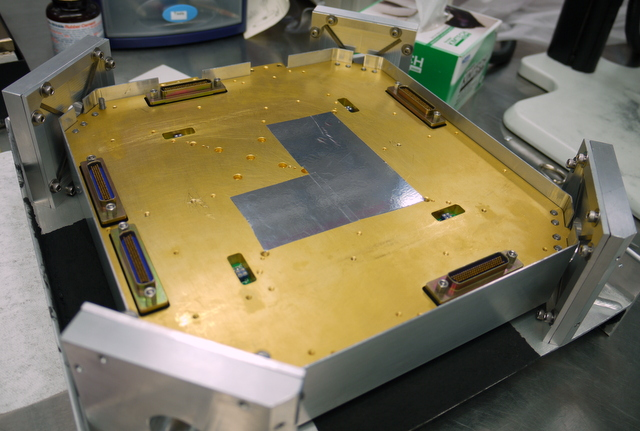
\includegraphics{drawings/ch5-focal-plane-back.pdf}
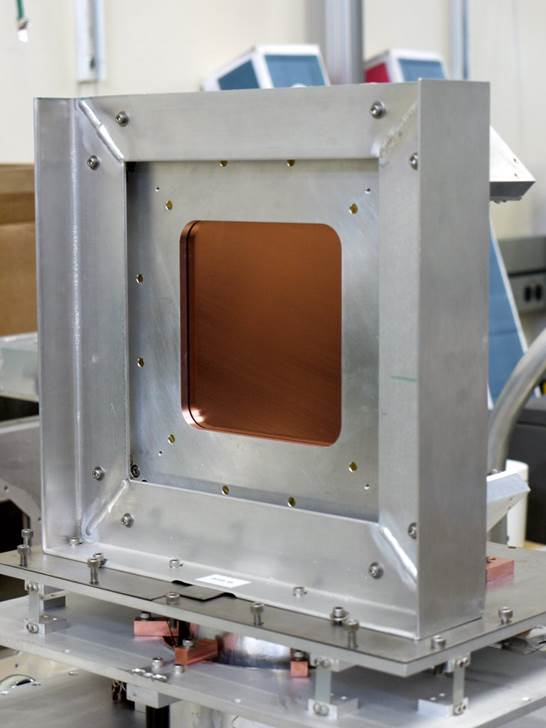
\includegraphics{drawings/ch5-focal-plane-cryostat.pdf}
\caption[Photograph of focal plane in cryostat]{
  Photographs showing how the focal plane is attached to the \SI{6}{\K} Cold Plate.
  \textbf{Left}
  Back view of the focal plane.
  At each corner the focal plane is bolted to a Ti-6Al-4V ``spider'', which are clamped into Al blocks (e.g. rectangles \textbf{A}).
  The blocks are then bolted to an Al frame, on which the blocks and focal plane are resting in the photograph.
  The Al frame has Berkeley Bock Black \cite{persky_review_1999} applied to it in an attempt to provide a surface on which stray infrared light will be absorbed other than the focal plane.
  Also visible are the 100-pin MDM connectors that the wires from the \MCE\ plug into (\textbf{B}).
  \textbf{Right}
  Photograph of the Al frame (\textbf{A}) and focal plane bolted onto the \SI{6}{\K} Cold Plate.
  The copper-colored area is the W1275 bandpass filter.
  This photograph was taken prior to the application of the Berkeley Bock Black.
  Also visiable in the photograph are the end-points of the Cu ropes that connect the PTC 2nd-stage cold head to the \SI{80}{\K} plate (\textbf{B}).
}
\label{fig:ch5-focal-plane-back}
\end{figure*}

Each sub-array is glued to a \SI{275}{\um} thick Si ``backshort'' wafer that has been micromachined to have the same outline as the sub-array and then covered with Au.
The glue was applied to the set of 26 holes in the detector wafer shown in \figref{fig:ch5-full-wafer}.
This wafer stack is then attached to an \SI{0.125}{\in} thick invar plate.
Invar was chosen because its thermal contraction upon cooling to \SI{4}{\K} and below is well-matched to Si \cite{ekin_experimental_2006}; choosing a material that is poorly matched to Si could result in breaking the Si stack upon cooling.
The wafer stack is attached to the invar plate with a thin layer of Apiezon-N thermal grease.
Upon cooling to cryogenic temperatures Apiezon N grease solidifies, so that the detector wafer will not slip along the invar.
Even at room temperature the grease is very thick so that if the back of the wafer stack is entirely covered with a layer of grease, the wafer will not slip under the influence of gravity if, e.g., it is stored facing horizontally in the cryostat while at room temperature.

The invar plates must be attached to the Al platter in a way that account for the differential thermal contraction between Al and Invar, while ensuring that the detectors are correctly aligned to the feedhorns.
This is done by aligning the invar, feedhorns, and Al platter to each other using stainless steel dowel pins.
Two pins align the feedhorns to the Al platter.
The dowel pins are inserted into the Al platter, with one matching hole and one matching slot in the feehorn array; a slot is used for one of the holes to avoid over-constraining the mechanical system.
Two additional pins align each invar plate feedhorn array to the Al platter.
Again a matching hole and slot are present in the invar, but in this case the slot is neccesary not only to avoid over-constraining the system but also to account for the differential thermal contraction between invar and Al.
The detector wafer is placed in the proper location on the invar platter using an alignment jig, and while the invar and grease have been warmed to \abt{\SI{30}{\celsius}}, a temperature at which the thermal grease becomes more viscous, making it easier to adjust the position of the wafer.
See \figref{fig:ch5-alignment-jig}.
This approach to mounting Si detector wafers on Invar and aligning to a feedhorn has been used by other instruments in the past, e.g. \cite{schwan_invited_2011}.

\begin{figure*}
\centering
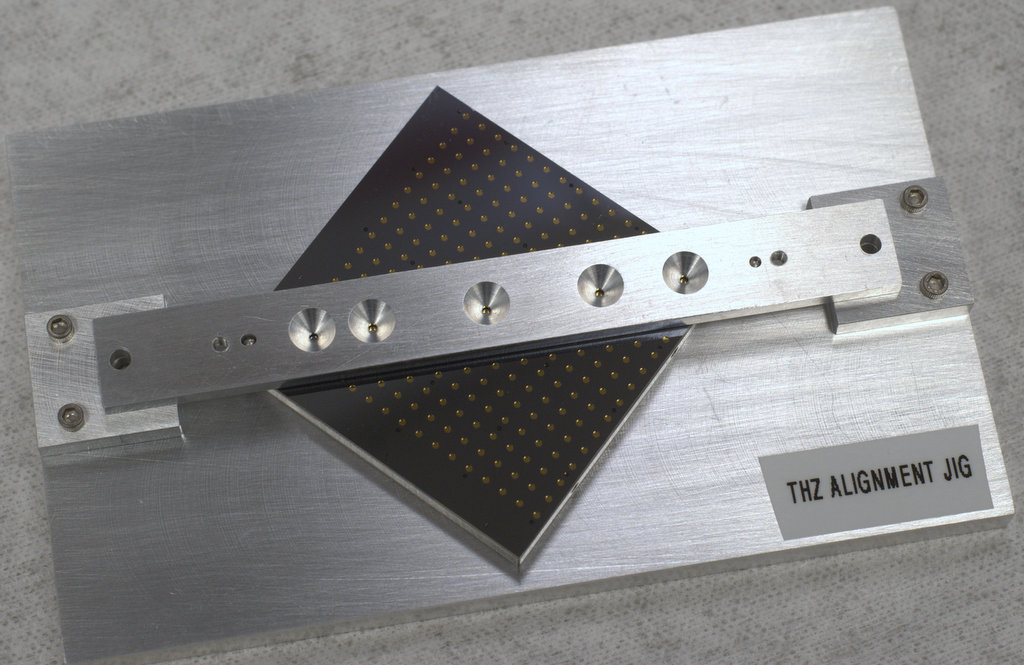
\includegraphics{drawings/ch5-alignment-jig.pdf}
\caption[Alignment jig]{
  Photograph of the alignment jig used to align the \Imager's sub-array to the invar plate.
  The invar plate and the metal bar are aligned to each other with dowel pins.
  The metal bar has conical cut-outs placed so that when detectors are aligned with them, the wafer is aligned properly to the invar.
  In order to make it easy to move the detector wafer stack to the proper location, the entire assembly is warmed to \SI{30}{\celsius}; at this temperature the thermal grease thins.
}
\label{fig:ch5-alignment-jig}
\end{figure*}

Four 100-wire woven PhBr wire harness run from \SI{300}{\K} to the focal plane, heat sunk along the way at the \SI{80}{\K} and \SI{6}{\K} stages.
These wires carry the readout signals to and from the \MCE.
Once they reach the focal plane a circuit board routes the wires to each sub-array.
One 100-wire harness caried the row-address wires and the circuit board routes the wires to all mutliplexing chips in series (32 chips for the full array).
The other four 100-wire harnesses each carry \SQUID\ bias and feedback wires for a single sub-array.

To aid in routing of the wires, each sub-array has two ``wiring chips'' associated with it, visible in \figref{fig:ch5-focal-plane-platter}, and shown in schematic form in \figref{fig:ch5-wiring-chip-schematic}.
These chips aid in routing row-address and detector bias wires.
On top of each wiring chip are four multiplexing chips as well as four ``interface'' chips which contain Nyquist inductors and shunt resistors for the detectors.

\begin{figure*}
\centering
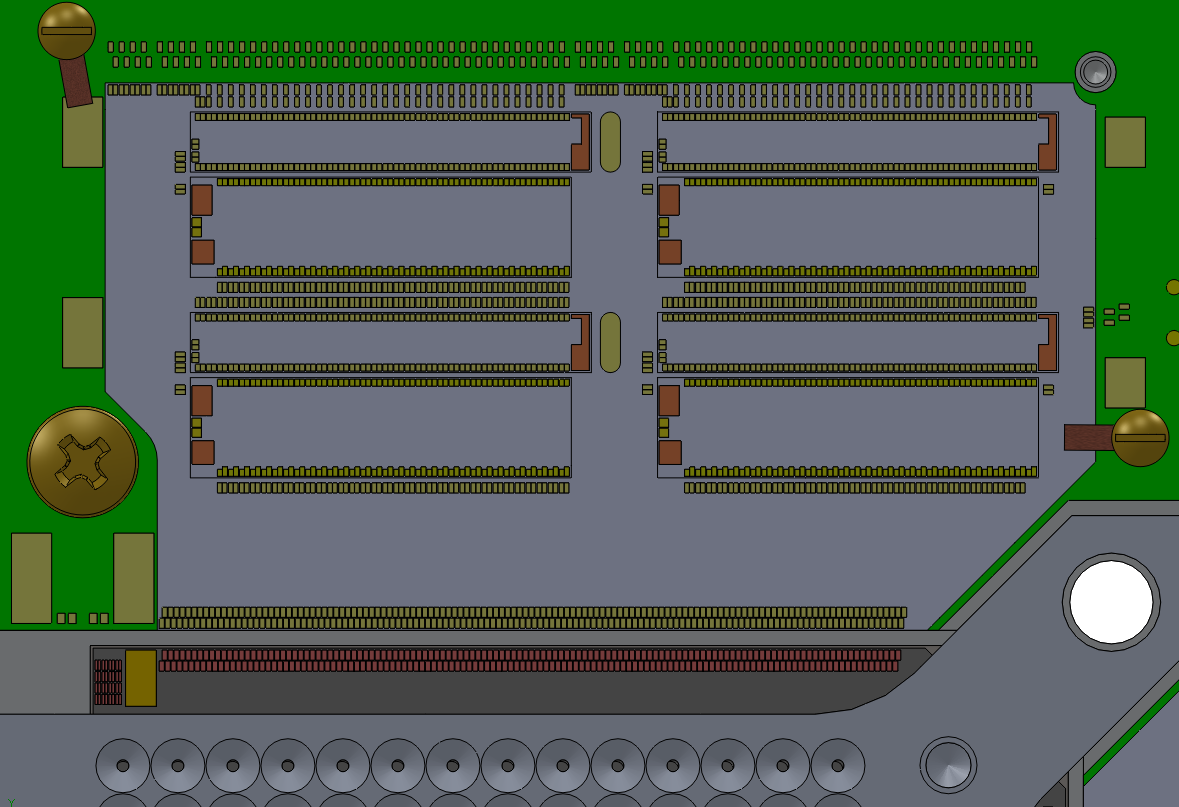
\includegraphics{drawings/ch5-wiring-chip-schematic.pdf}
\caption[Wiring chip schematic]{
  Schematic showing close-up view of the wiring chips with multiplexing and interface chips on top.
}
\label{fig:ch5-wiring-chip-schematic}
\end{figure*}

\begin{figure*}
\centering
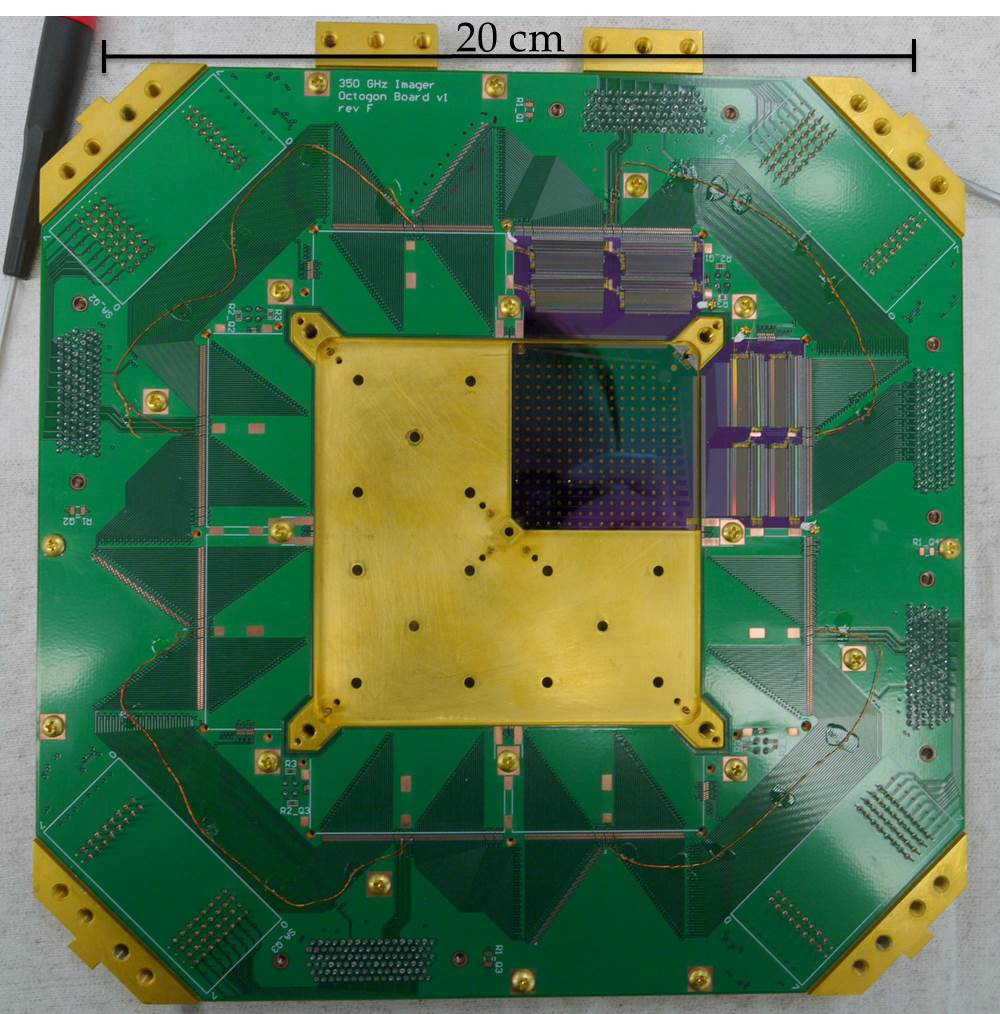
\includegraphics{drawings/ch5-focal-plane-platter.pdf}
\caption[Focal plane during assembly]{
  Photograph of the focal plane platter while being assembled.
  The platter was machined out of Al 6061 and then Au-plated.
  The green circuit board routes the 500 PhBr wires running from room temperature to the multiplexing and interface chips.
  The wiring chips (with multiplexing and interface chips on top) are labeled \textbf{A}, while the 251-detector sub-array is labeled \textbf{B}.
}
\label{fig:ch5-focal-plane-platter}
\end{figure*}

\section{Predicted Noise} \label{sec:ch5-predicted-noise}

Using the targeted value of $G$ we can predict the total noise on the detectors as well as the expected \NETD\ in video images.
As discussed in \sectionref{sec:ch3-tes-noise}, intrinsic detector noise should be dominated by thermal fluctuation noise, given by
\begin{equation}
  S^2_{TFN} = 4 k_B T_0^2 G F(T_0, T_b).
\end{equation}
Using $G = \SI{3.8}{\nW\per\K}$, $T_0 = \SI{1.2}{\K}$, and $F = 0.83$ leads to $S_{TFN} = \Pnoisef{0.5}$.
This is \SI{60}{\percent} of \sectionref{sec:ch4-opt-eff}'s predicted photon noise of \Pnoisef{0.85}.
Summing the two noise sources in quadrature gives for the total noise (referred to power absorbed in the detector) $S_{tot} = \Pnoisef{1.0}$.

xxx need discussion of NETD, but want to write that section in ch2 first

\section{Acknowledgments}

Hsiao-Mei (Sherry) Cho fabricated the detectors and wiring chips, as well as providing much useful advice during the design and layout of both.
The interface chips were designed --- and spares kindly donated --- by the Atacama B-Mode Search team.
Jeff Van Lanen fabricated the backshort wafers and the Quantum Sensors Project \SQUID\ fabrication team made the multiplexing chips.
Colin Fitzgerald performed all wire bonding.
